\documentclass[DaoFP]{subfiles}
\begin{document}
\setcounter{chapter}{9}

\chapter{伴随}

雕塑家去除无关的石头,直到雕塑显现。数学家抽象无关的细节,直到模式显现。

我们能够使用它们的映射入和映射出性质来定义许多构造。这些性质又可以简洁地写成hom集之间的同构。这种hom集之间的自然同构模式被称为伴随(adjunction),一旦被识别,几乎无处不在。

\section{柯里化伴随}

指数的定义是伴随的经典例子,它关联了映射出和映射入。每个从积中映射出的映射都对应一个唯一的映射入指数的映射:
\[  \mathcal{C}(e \times a, b ) \cong  \mathcal{C} (e, b^a)  \]
对象$b$在左侧扮演焦点的角色;对象$e$在右侧成为观察者。

我们可以发现两个函子在起作用。它们都由$a$参数化。在左侧,我们有应用于$e$的积函子$(- \times a)$。在右侧,我们有应用于$b$的指数函子$(-)^a$。

如果我们将这些函子写成:
\[ L_a e = e \times a \]
\[ R_a b = b^a \]
那么自然同构
\[ \mathcal{C}(L_a e, b) \cong \mathcal{C}(e, R_a b) \]
被称为它们之间的伴随。

在分量中,这个同构告诉我们,给定一个映射$\phi \in \mathcal{C}(L_a e, b)$,存在一个唯一的映射$\phi^T \in \mathcal{C}(e, R_a b)$,反之亦然。这些映射有时被称为彼此的\emph{转置}(transpose)---这个术语来自矩阵代数。

伴随的简写符号是$L \dashv R$。将积函子代入$L$,指数函子代入$R$,我们可以将柯里化伴随简洁地写成:

\[ (- \times a) \dashv (-)^a \]

指数对象$b^a$有时被称为\index{内部hom}\emph{内部hom}(internal hom),并写作$[a, b]$。这与\emph{外部hom}(external hom)形成对比,后者是集合$\cat C (a, b)$。外部hom\emph{不是} $\cat C$中的对象(除非$\cat C$本身是$\Set$)。使用这种符号,柯里化伴随可以写成:
\[  \mathcal{C}(e \times a, b) \cong  \mathcal{C} (e, [a, b])  \]
这种伴随成立的范畴被称为笛卡尔闭范畴。

由于函数在每个编程语言中扮演核心角色,笛卡尔闭范畴构成了所有编程模型的基础。我们将指数$b^a$解释为函数类型$a \to b$。

这里$e$扮演外部环境的角色---lambda演算中的$\Gamma$。$\cat C(\Gamma \times a, b)$中的态射被解释为在环境$\Gamma$中扩展了一个类型为$a$的变量的类型为$b$的表达式。因此,函数类型$a \to b$表示一个可能从其环境中捕获类型为$e$的值的闭包。

顺便提一下,(小)范畴的范畴$\mathbf{Cat}$也是笛卡尔闭的,这反映在积范畴和函子范畴之间的伴随中,使用了相同的内部hom符号:
\[ \mathbf{Cat} (\cat A \times \cat B, \cat C) \cong \mathbf{Cat} (\cat A, [\cat B, \cat C]) \]
这里,两边都是自然变换的集合。

\section{和与积的伴随}

Currying伴随关系涉及两个自函子,但伴随关系可以很容易地推广到不同范畴之间的函子。让我们先看一些例子。

\subsection{对角函子}

和类型与积类型是通过双射定义的,其中一边是单个箭头,另一边是一对箭头。一对箭头可以看作是积范畴中的单个箭头。

为了探讨这一想法,我们需要定义对角函子 $\Delta$,它是从 $\mathcal{C}$ 到 $\mathcal{C} \times \mathcal{C}$ 的特殊映射。它取一个对象 $x$ 并复制它,生成一对对象 $\langle x, x \rangle$。它还取一个箭头 $f$ 并复制它 $\langle f, f \rangle$。

有趣的是,对角函子与我们之前见过的常函子有关。常函子可以被视为一个双变量函子——它只是忽略第二个变量。我们在Haskell定义中见过这一点:
\begin{haskell}
data Const c a = Const c
\end{haskell}

为了看到这种联系,让我们将积范畴 $\mathcal{C} \times \mathcal{C}$ 视为函子范畴 $[ \mathbf{2}, \mathcal{C}]$,换句话说,$\mathbf{Cat}$ 中的指数对象 $\mathcal{C}^{ \mathbf{2}}$。实际上,从 $\mathbf{2}$(有两个对象的简笔范畴)的函子选择一对对象——这等价于积范畴中的单个对象。

一个函子 $\mathcal{C} \to [\mathbf{2}, \mathcal{C}]$ 可以反curry化为 $\mathcal{C} \times \mathbf{2} \to  \mathcal{C}$。对角函子忽略第二个参数,即来自 $\mathbf{2}$ 的参数:无论第二个参数是 $1$ 还是 $2$,它都做同样的事情。这正是常函子所做的。这就是为什么我们对两者使用相同的符号 $\Delta$。

顺便说一下,这个论证可以很容易地推广到任何索引范畴,而不仅仅是 $\mathbf{2}$。

\subsection{和伴随}

回想一下,和类型是由其映射出属性定义的。从和 $a + b$ 出来的箭头与分别从 $a$ 和 $b$ 出来的箭头对之间存在一一对应关系。在hom集的术语中,我们可以写成:
\[  \mathcal{C} (a + b, x) \cong \mathcal{C}( a , x) \times \mathcal{C}( b , x)\]
其中右边的积只是集合的笛卡尔积,即对的集合。此外,我们之前已经看到这个双射在 $x$ 上是自然的。

我们知道,一对箭头是积范畴中的单个箭头。因此,我们可以将右边的元素视为 $\mathcal{C} \times \mathcal{C}$ 中从对象 $\langle a, b \rangle$ 到对象 $\langle x, x \rangle$ 的箭头。后者可以通过对角函子 $\Delta$ 作用于 $x$ 得到。我们有:

\[  \mathcal{C} (a + b, x) \cong (\mathcal{C} \times \mathcal{C})( \langle a, b \rangle , \Delta x)\]
这是两个不同范畴中hom集之间的双射。它满足自然性条件,因此是一个自然同构。

我们也可以在这里发现一对函子。在左边,我们有一个函子,它取一对对象 $\langle a, b \rangle$ 并生成它们的和 $a + b$:
\[ (+) \colon \mathcal{C} \times \mathcal{C} \to \mathcal{C}\]
在右边,我们有对角函子 $\Delta$ 朝相反的方向:
\[ \Delta \colon \mathcal{C} \to  \mathcal{C} \times \mathcal{C} \]
总的来说,我们有一对范畴之间的一对函子:
\[
 \begin{tikzcd}
  \mathcal{C}
   \arrow[rr, bend right, "\Delta"']
  &&
  \mathcal{C} \times \mathcal{C}
 \arrow[ll, bend right, "(+)"']
  \end{tikzcd}
\]
以及hom集之间的同构:
\[
 \begin{tikzcd}
a + b
\arrow[d, bend right, red, dashed]
\arrow[d, dashed]
\arrow[d, bend left, blue, dashed]
  &&
 \langle a , b \rangle
\arrow[d, bend right, red, dashed]
\arrow[d, dashed]
\arrow[d, bend left, blue, dashed]
 \arrow[ll, bend right, "(+)"']
 \\
 x
   \arrow[rr, bend right, "\Delta"']
 &&
 \langle x, x \rangle
  \end{tikzcd}
\]
换句话说,我们有伴随关系:
\[ (+) \dashv \Delta \]


\subsection{积伴随}

我们可以将相同的推理应用于积的定义。这次我们有一对箭头与映射到积之间的自然同构。

\[  \mathcal{C} (x, a) \times \mathcal{C}(x, b) \cong  \mathcal{C} (x, a \times b)  \]
将箭头对替换为积范畴中的箭头,我们得到:

\[  (\mathcal{C} \times \mathcal{C})( \Delta x,  \langle a, b \rangle ) \cong  \mathcal{C} (x, a \times b)  \]
这是两个朝相反方向的函子:
\[
 \begin{tikzcd}
  \mathcal{C} \times \mathcal{C}
  \arrow[rr, bend right, "(\times)"']
  &&
  \mathcal{C}
  \arrow[ll, bend right, "\Delta"']
  \end{tikzcd}
\]
以及hom集的同构:

\[
 \begin{tikzcd}
 \langle x, x \rangle
\arrow[d, bend right, red, dashed]
\arrow[d, dashed]
\arrow[d, bend left, blue, dashed]
  &&
  x
\arrow[d, bend right, red, dashed]
\arrow[d, dashed]
\arrow[d, bend left, blue, dashed]
 \arrow[ll, bend right, "\Delta"']
 \\
 \langle a , b \rangle
   \arrow[rr, bend right, "(\times)"']
 &&
 a \times b
  \end{tikzcd}
\]
换句话说,我们有伴随关系:
\[ \Delta \dashv (\times) \]

\subsection{分配律}

在双笛卡尔闭范畴中,积对和具有分配性。我们已经使用泛构造看到了证明的一个方向。伴随关系与Yoneda引理相结合,为我们提供了更强大的工具来解决这个问题。

我们想要展示自然同构:
\[(b + c) \times a \cong b \times a + c \times a \]
与其直接证明这个恒等式,不如展示从两边到任意对象 $x$ 的映射是同构的:
\[  \mathcal{C} ((b + c) \times a, x) \cong \mathcal{C}(b \times a + c \times a, x) \]
左边是积的映射,因此我们可以对其应用currying伴随关系:
\[  \mathcal{C} ((b + c) \times a, x) \cong \mathcal{C}(b + c, x^a) \]
这给出了和的映射,根据和伴随关系,它同构于两个映射的积:
\[  \mathcal{C}(b + c, x^a) \cong \mathcal{C}(b, x^a) \times \mathcal{C}(c, x^a)\]
我们现在可以对两个分量应用currying伴随关系的逆:
\[  \mathcal{C}(b, x^a) \times \mathcal{C}(c, x^a) \cong \mathcal{C}(b \times a, x) \times \mathcal{C}(c \times a, x)\]
使用和伴随关系的逆,我们得到最终结果:
\[ \mathcal{C}(b \times a, x) \times \mathcal{C}(c \times a, x) \cong \mathcal{C}(b \times a + c \times a, x) \]

这个证明中的每一步都是自然同构,因此它们的组合也是自然同构。根据Yoneda引理,分配律左右两边的两个对象因此是同构的。

这个陈述的一个更简短的证明来自我们即将讨论的左伴随的性质。

\section{函子之间的伴随关系}

一般来说,伴随关系描述的是在两个范畴之间反向进行的两个函子之间的关系。左函子
\[ L \colon \mathcal{D} \to \mathcal{C}\]
和右函子:
\[ R \colon \mathcal{C} \to  \mathcal{D} \]
伴随关系 $L \dashv R$ 被定义为两个 hom-集之间的自然同构。
\[  \mathcal{C} (L x, y) \cong \mathcal{D}( x , R y)\]
换句话说,我们有一族集合之间的可逆函数:
\[ \phi_{x y} \colon  \mathcal{C} (L x, y) \to \mathcal{D}( x , R y) \]
在 $x$ 和 $y$ 上都是自然的。例如,在 $y$ 上的自然性意味着,对于任何 $f \colon y \to y'$,以下图表交换:
\[
 \begin{tikzcd}
 \mathcal{C}(L x, y)
 \arrow[d, leftrightarrow, "\phi_{x y}"]
 \arrow[r, "{\mathcal{C}(L x, f)}"]
 &
 \mathcal{C}(L x, y')
  \arrow[d, leftrightarrow, "\phi_{x y'}"]
 \\
 \mathcal{D}(x, R y)
 \arrow[r, "{\mathcal{D}(x, R f)}"]
& \mathcal{D}(x, R y')
 \end{tikzcd}
\]
或者,考虑到通过 hom-函子提升箭头与后复合相同:
\[
 \begin{tikzcd}
 \mathcal{C}(L x, y)
 \arrow[d, leftrightarrow, "\phi_{x y}"]
 \arrow[r, "f \circ -"]
 &
 \mathcal{C}(L x, y')
  \arrow[d, leftrightarrow, "\phi_{x y'}"]
 \\
 \mathcal{D}(x, R y)
 \arrow[r, "R f \circ -"]
& \mathcal{D}(x, R y')
 \end{tikzcd}
\]
双头箭头可以沿任一方向遍历(向上时使用 $\phi^{-1}_{x y}$),因为它们是同构的分量。

图示上,我们有两个函子:
\[
 \begin{tikzcd}
  \mathcal{C}
  \arrow[rr, bend right, "R"']
  &&
  \mathcal{D}
  \arrow[ll, bend right, "L"']
  \end{tikzcd}
\]
并且,对于任何一对 $x$ 和 $y$,有两个同构的 hom-集:
\[
 \begin{tikzcd}
L x
\arrow[d, bend right, red, dashed]
\arrow[d, dashed]
\arrow[d, bend left, blue, dashed]
  &&
  x
\arrow[d, bend right, red, dashed]
\arrow[d, dashed]
\arrow[d, bend left, blue, dashed]
 \arrow[ll, bend right, "L"']
 \\
y
   \arrow[rr, bend right, "R"']
 &&
 R y
  \end{tikzcd}
\]
这些 hom-集来自两个不同的范畴,但集合就是集合。我们说 $L$ 是 $R$ 的左伴随,或者 $R$ 是 $L$ 的右伴随。

在 Haskell 中,这个的简化版本可以编码为一个多参数类型类:
\begin{haskell}
class (Functor left, Functor right) => Adjunction left right where
  ltor :: (left x -> y) -> (x -> right y)
  rtol :: (x -> right y) -> (left x -> y)
\end{haskell}
它需要在文件顶部添加以下编译指示:
\begin{haskell}
{-# language MultiParamTypeClasses #-}
\end{haskell}

因此,在双笛卡尔范畴中,和是对角函子的左伴随;积是其右伴随。我们可以非常简洁地写出这一点(或者我们可以用现代版本的楔形文字将其印在粘土上):
\[ (+) \dashv \Delta \dashv (\times) \]

\begin{exercise}
画出见证伴随函数 $\phi_{x y}$ 在 $x$ 上自然性的交换方块。
\end{exercise}

\begin{exercise}
伴随公式左侧的 hom-集 $\mathcal{C} (L x, y)$ 表明 $L x$ 可以被视为某个函子(共预层)的表示对象。这个函子是什么?提示:它将 $y$ 映射到一个集合。这个集合是什么?
\end{exercise}

\begin{exercise}
反过来,预层 $P$ 的表示对象 $a$ 定义为:
\[P x \cong \mathcal{D}(x, a)\]
在伴随公式中,$R y$ 是哪个预层的表示对象。
\end{exercise}

\section{极限与余极限作为伴随}

极限的定义也涉及到同态集之间的自然同构:
\[ [\cat J, \mathcal{C}](\Delta_x, D)  \cong \mathcal{C}(x, \text{Lim} D) \]
左边的同态集位于函子范畴中。它的元素是锥,或者是常函子 $\Delta_x$ 与图表函子 $D$ 之间的自然变换。右边的同态集位于 $\mathcal{C}$ 中。

在所有极限存在的范畴中,我们有以下两个函子之间的伴随关系:
\[ \Delta_{(-)} \colon \mathcal{C} \to  [\cat J, \mathcal{C}] \]
和:
\[ \text{Lim}{(-)} \colon  [\cat J, \mathcal{C}] \to \mathcal{C} \]

对偶地,余极限由以下自然同构描述:
\[ [\cat J, \mathcal{C}](D, \Delta_x)  \cong \mathcal{C}( \text{Colim} D, x) \]
我们可以用一个简洁的公式来表示这两个伴随关系:
\[ \text{Colim} \dashv \Delta \dashv \text{Lim}\]

特别地,由于积范畴 $\cat C \times \cat C$ 等价于 $\cat C^2$,即函子范畴 $[\mathbf{2}, \cat C]$,我们可以将积和余积重写为极限和余极限:
\[ [\mathbf{2}, \cat C](\Delta_x, \langle a, b \rangle) \cong \cat C(x, a \times b) \]
\[ \cat C( a + b, x) \cong [\mathbf{2}, \cat C]( \langle a, b \rangle, \Delta_x) \]
其中 $\langle a, b \rangle$ 表示一个图表,它是函子 $D \colon \mathbf{2} \to \cat C$ 在 $\mathbf{2}$ 的两个对象上的作用。

\section{伴随的单位与余单位}

我们通过等式来比较箭头,但在比较对象时,我们更倾向于使用同构。

然而,当我们处理函子时,问题就出现了。一方面,它们是函子范畴中的对象,因此同构是合适的选择;另一方面,它们是$\mathbf{Cat}$中的箭头,所以也许可以用等式来比较它们?

为了阐明这一困境,我们应该问自己\emph{为什么}我们使用等式来比较箭头。这并不是因为我们喜欢等式,而是因为在集合中,除了比较元素的等式之外,我们别无他法。同态集中的两个元素要么相等,要么不相等,仅此而已。

但在$\mathbf{Cat}$中情况并非如此,我们知道,$\mathbf{Cat}$是一个$2$-范畴。在这里,同态集本身具有范畴的结构——函子范畴。在$2$-范畴中,我们有箭头之间的箭头,因此特别是,我们可以定义箭头之间的同构。在$\mathbf{Cat}$中,这些将是函子之间的自然同构。

然而,尽管我们可以选择用同构来替换箭头等式,$\mathbf{Cat}$中的范畴法则仍然表示为等式。例如,函子$F$与恒等函子的复合\emph{等于}$F$,结合性也是如此。在这种法则“严格”满足的$2$-范畴中,称为\emph{严格}$2$-范畴,而$\mathbf{Cat}$就是严格$2$-范畴的一个例子。

但在比较范畴时,我们有更多的选择。范畴是$\mathbf{Cat}$中的对象,因此可以定义范畴的同构为一对函子$L$和$R$:
\[
 \begin{tikzcd}
  \mathcal{C}
  \arrow[rr, bend right, "R"']
  \arrow[loop, "\text{Id}_{ \mathcal{C}} "']
  &&
  \mathcal{D}
  \arrow[ll, bend right, "L"']
  \arrow[loop, "\text{Id}_{ \mathcal{D}} "']
  \end{tikzcd}
\]
使得:
\begin{align*}
L \circ R = \text{Id}_{ \mathcal{C}} \\
\text{Id}_{ \mathcal{D}} = R \circ L 
\end{align*}
然而,这个定义涉及函子的等式。更糟糕的是,作用于对象时,它涉及对象的等式:
\begin{align*}
 L (R x) = x \\
 y = R (L y)
\end{align*}
这就是为什么更合适的是讨论范畴的\emph{等价}这一较弱的概念,其中等式被同构取代:
\begin{align*}
L \circ R \cong \text{Id}_{ \mathcal{C}} \\
 \text{Id}_{ \mathcal{D}} \cong R \circ L 
\end{align*}
在对象上,范畴的等价意味着往返操作产生的对象与原始对象同构,而不是相等。在大多数情况下,这正是我们想要的。

伴随也定义为方向相反的一对函子,因此询问往返操作的结果是有意义的。

定义伴随的同构适用于任何对象对$x$和$y$
\[  \mathcal{C} (L x, y) \cong \mathcal{D}( x , R y)\]
因此,特别是,如果我们用$L x$替换$y$,它也适用
\[  \mathcal{C} (L x, L x) \cong \mathcal{D}( x , R (L x))\]
我们现在可以使用Yoneda技巧,在左侧选择恒等箭头$id_{L x}$。同构将其映射到右侧的唯一箭头,我们称之为$\eta_x$:
\[ \eta_x \colon x \to R ( L x) \]
这个映射不仅对每个$x$都有定义,而且在$x$上是自然的。自然变换$\eta$称为伴随的\emph{单位}。如果我们注意到左侧的$x$是恒等函子作用于$x$的结果,我们可以写成:
\[ \eta \colon \text{Id}_{\mathcal{D}} \to R \circ L \]

例如,让我们评估余积伴随的单位:
\[  \mathcal{C} (a + b, x) \cong (\mathcal{C} \times \mathcal{C})( \langle a, b \rangle , \Delta x)\]
通过用$a + b$替换$x$。我们得到:
\[ \eta_{\langle a, b \rangle} \colon \langle a, b \rangle \to \Delta(a + b) \]
这是一对箭头,正是两个注入$\langle \text{Left}, \text{Right} \rangle$。

我们可以通过用$R y$替换$x$来做类似的技巧:
\[  \mathcal{C} (L (R y), y) \cong \mathcal{D}( R y , R y)\]
对应于右侧的$id_{R y}$,我们在左侧得到一个箭头:
\[ \varepsilon_y \colon L (R y) \to y \]
这些箭头形成另一个自然变换,称为伴随的\emph{余单位}:
\[ \varepsilon \colon L \circ R \to \text{Id}_{\mathcal{C}}  \]

注意,如果这两个自然变换是可逆的,它们将见证范畴的等价。但即使它们不是,这种“半等价”在范畴论的背景下仍然非常有趣。

例如,让我们评估积伴随的余单位:
\[  (\mathcal{C} \times \mathcal{C})( \Delta x,  \langle a, b \rangle ) \cong  \mathcal{C} (x, a \times b)  \]
通过用$a \times b$替换$x$。我们得到:
\[ \varepsilon_{\langle a, b \rangle} \colon \Delta (a \times b) \to \langle a, b \rangle \]
这是一对箭头,正是两个投影$\langle \text{fst}, \text{snd} \rangle$。

\begin{exercise}
推导余积伴随的余单位和积伴随的单位。
\end{exercise}

\subsection{三角恒等式}

我们可以使用单位/余单位对来表述伴随的等价定义。为此,我们从一对自然变换开始:
\begin{align*}
\eta \colon \text{Id}_{\mathcal{D}} \to R \circ L \\
\varepsilon \colon L \circ R \to \text{Id}_{\mathcal{C}} 
\end{align*}
并施加额外的\emph{三角恒等式}。

这些恒等式可以通过伴随的标准定义推导出来,注意到$\eta$可以用来用复合$R \circ L$替换恒等函子,从而让我们在任何恒等函子起作用的地方插入$R \circ L$。

类似地,$\varepsilon$可以用来消除复合$L \circ R$(即用恒等替换它)。

因此,例如,从$L$开始:
\[ L = L \circ \text{Id}_{\mathcal{D}} \xrightarrow{L \circ \eta} L \circ R \circ L \xrightarrow{\varepsilon \circ L} \text{Id}_{\mathcal{C}} \circ L = L \]
在这里,我们使用了自然变换的水平复合,其中一个变换是恒等变换(也称为whiskering)。

第一个三角恒等式是这一系列变换结果等于恒等自然变换的条件。图示如下:

\[
 \begin{tikzcd}
 L
 \arrow[r, "L \circ \eta"]
 \arrow[rd, "id_L"']
 & L \circ R \circ L
 \arrow[d, "\varepsilon \circ L"]
 \\
 & L
  \end{tikzcd}
\]

类似地,我们希望以下一系列自然变换也复合为恒等:
\[ R = \text{Id}_{\mathcal{D}} \circ R \xrightarrow{\eta \circ R} R \circ L \circ R \xrightarrow{R \circ \varepsilon} R \circ \text{Id}_{\mathcal{C}} = R \]
或图示如下:
\[
 \begin{tikzcd}
 R
 \arrow[r, "\eta \circ R"]
 \arrow[rd, "id_R"']
 & R \circ L \circ R
 \arrow[d, "R \circ \varepsilon"]
 \\
 & R
  \end{tikzcd}
\]

事实证明,伴随可以等价地用两个自然变换$\eta$和$\varepsilon$来定义,满足三角恒等式:
\begin{align*}
(\varepsilon \circ L) \cdot (L \circ \eta) = id_L \\
(R \circ \varepsilon) \cdot (\eta \circ R) = id_R
\end{align*}

从这些恒等式中,可以很容易地恢复同态集的映射。例如,让我们从一个箭头$f \colon x \to R y$开始,它是$\mathcal{D}( x , R y)$的一个元素。我们可以将其提升为
\[L f \colon L x \to L (R y)\]
然后我们可以使用$\eta$将复合$L \circ R$折叠为恒等。结果是一个箭头$L x \to y$,它是$ \mathcal{C} (L x, y)$的一个元素。

使用单位和余单位定义的伴随在某种意义上更通用,因为它可以转化为任意的$2$-范畴设置。

\begin{exercise}
给定一个箭头$g \colon L x \to y$,使用$\varepsilon$和$R$是函子的事实,实现一个箭头$x \to R y$。提示:从对象$x$开始,看看如何通过一个中转点从那里到达$R y$。
\end{exercise}

\subsection{柯里化伴随的单位与余单位}

让我们计算柯里化伴随的单位和余单位:
\[  \mathcal{C}(e \times a, b ) \cong  \mathcal{C} (e, b^a)  \]
如果我们用$e \times a$替换$b$,我们得到
\[  \mathcal{C}(e \times a, e \times a ) \cong  \mathcal{C} (e, (e \times a)^a)  \]
对应于左侧的恒等箭头,我们在右侧得到伴随的单位:
\[ \eta \colon e \to (e \times a)^a \]
这是积构造器的柯里化版本。在Haskell中,我们写成:
\begin{haskell}
unit :: e -> (a -> (e, a))
unit = curry id
\end{haskell}

余单位更有趣。用$b^a$替换$e$,我们得到:
\[  \mathcal{C}(b^a \times a, b ) \cong  \mathcal{C} (b^a, b^a)  \]
对应于右侧的恒等箭头,我们得到:
\[ \varepsilon \colon b^a \times a \to b \]
这是函数应用箭头。

在Haskell中:
\begin{haskell}
counit :: (a -> b, a) -> b
counit = uncurry id
\end{haskell}

当伴随在两个自函子之间时,我们可以使用单位和余单位写出Haskell中的替代定义:
\begin{haskell}
class (Functor left, Functor right) => 
  Adjunction left right | left -> right, right -> left where
    unit   :: x -> right (left x)
    counit :: left (right x) -> x
\end{haskell}
额外的两个子句\hask{left -> right}和\hask{right -> left}告诉编译器,在使用伴随的实例时,一个函子可以从另一个函子派生出来。这个定义需要以下编译扩展:
\begin{haskell}
{-# language MultiParamTypeClasses #-}
{-# LANGUAGE FunctionalDependencies #-}
\end{haskell}

形成柯里化伴随的两个函子可以写成:
\begin{haskell}
data L r x = L (x, r)    deriving (Functor, Show)
data R r x = R (r -> x)  deriving Functor
\end{haskell}
柯里化的\hask{Adjunction}实例是:
\begin{haskell}
instance Adjunction (L r) (R r) where
  unit x = R (\r -> L (x, r)) 
  counit (L (R f, r)) = f r
\end{haskell}
第一个三角恒等式表明以下多态函数:
\begin{haskell}
triangle :: L r x -> L r x
triangle = counit . fmap unit
\end{haskell}
是恒等函数,第二个也是如此:
\begin{haskell}
triangle' :: R r x -> R r x
triangle' = fmap counit . unit
\end{haskell}
注意,这两个函数需要使用函数依赖才能正确定义。三角恒等式无法在Haskell中表达,因此伴随的实现者需要证明它们。
\begin{exercise}
测试柯里化伴随的第一个三角恒等式的几个例子。以下是一个例子:
\begin{haskell}
triangle (L (2, 'a'))
\end{haskell}
\end{exercise}

\begin{exercise}
你如何测试柯里化伴随的第二个三角恒等式?提示:\hask{triangle'}的结果是一个函数,因此你无法显示它,但你可以调用它。
\end{exercise}

\section{使用通用箭头的伴随}

我们已经看到了使用同态集同构定义的伴随,以及使用单位/余单位对定义的另一种方式。事实证明,只要满足某些通用性条件,我们可以仅使用这对中的一个元素来定义伴随。为了理解这一点,我们将构建一个新范畴,其对象是箭头。

我们之前已经见过这样一个范畴的例子——切片范畴 $\cat C/ c$,它收集了所有收敛于 $c$ 的箭头。这样的范畴描述了从 $\cat C$ 中每个可能的角度观察对象 $c$ 的情况。

\subsection{逗号范畴}
在处理伴随时:
\[  \mathcal{C} (L d, c) \cong \mathcal{D}( d , R c)\]
我们是从由函子 $L$ 定义的更窄的视角观察对象 $c$。将 $L$ 视为在 $\cat C$ 内部定义 $\cat D$ 的模型。我们感兴趣的是从这个模型的视角观察 $c$ 的情况。描述这种视角的箭头形成了逗号范畴 $L/c$。

\[
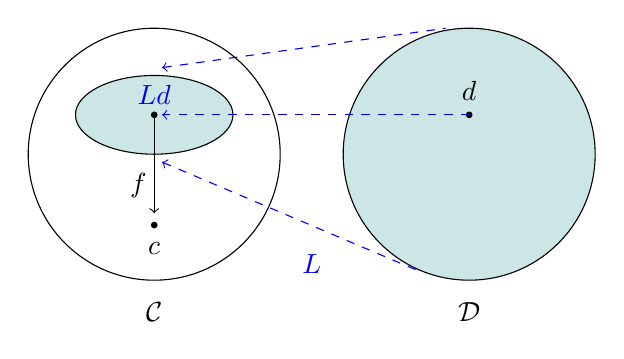
\begin{tikzpicture}
  \def\Xa{2.0};
  \def\Xb{-2.0};
  
  \def\Ytip{-0.9};
  \def\Yo{0.5}; % oval
  \def\Yb{-2.0}; % labels
         \draw (\Xa, 0)[fill=blue!50!green!20]  ellipse (1.6 and 1.6);
         \draw (\Xb , 0) ellipse (1.6 and 1.6);
         % oval
         \draw (\Xb , \Yo)[fill=blue!50!green!20] ellipse (1 and 0.5);
         
        % apex
        \filldraw (\Xb, \Ytip) circle (1pt);
        \node at ( \Xb, \Ytip - 0.3) { $c$ };
        
        % image
        \filldraw (\Xa, \Yo) circle (1pt);
        \node at ( \Xa, \Yo + 0.3) { $d$ };
        
	% middle of the cone
	\draw[->] (\Xb, \Yo) -- (\Xb, \Ytip + 0.15);
	\node at (\Xb - 0.2, \Ytip + 0.5) {$f$};
        	% sides of the cone
	%\draw (\Xb, \Ytip) -- (\Xb + 0.95, \Yo - 0.15);
	%\draw (\Xb, \Ytip) -- (\Xb - 0.95, \Yo - 0.15);

        % categories
        \node at (\Xa, \Yb) { $\mathcal D$ };
        \node at (\Xb, \Yb) { $\mathcal C$ };
        \node[blue] at (0, \Yb + 0.6) { $L$ };

        % functor middle
        \filldraw (\Xb, \Yo) circle (1pt);
        \node[blue] at ( \Xb, \Yo + 0.25) { $L d$ };
	\draw[->, blue, dashed] (\Xa, \Yo) -- (\Xb + 0.1, \Yo);
	% functor 
	\draw [<-, blue, dashed] (\Xb + 0.1, \Yo + 0.6)   --   (\Xa - 0.3, \Yo + 1.1);
	\draw [<-,blue, dashed] (\Xb + 0.1, \Yo - 0.6) -- (\Xa - 0.6, \Ytip - 0.6);
\end{tikzpicture}
\]

在\index{逗号范畴}\emph{逗号范畴} $L/c$ 中,一个对象是一个对 $\langle d, f \rangle$,其中 $d$ 是 $\cat D$ 的一个对象,$f \colon L d \to c$ 是 $\cat C$ 中的一个箭头。

从 $\langle d, f \rangle$ 到 $\langle d', f' \rangle$ 的态射是一个箭头 $h \colon d \to d'$,使得左边的图表交换:
\[
 \begin{tikzcd}
 L d
 \arrow[rd, "f"']
 \arrow[rr, "L h"]
 && L d'
 \arrow[ld, "f'"]
 \\
 &c
  \end{tikzcd}
 \hspace{30pt}
\begin{tikzcd}
 d
 \arrow[rr, "h"]
 && d'
  \end{tikzcd}
\]

\subsection{通用箭头}

从 $L$ 到 $c$ 的通用箭头定义为逗号范畴 $L / c$ 中的终对象。让我们拆解这个定义。$L/c$ 中的终对象是一个对 $\langle t, \tau \rangle$,具有从任何对象 $\langle d, f \rangle$ 的唯一态射。这样的态射是一个箭头 $h \colon d \to t$,满足交换条件:
\[
 \begin{tikzcd}
 L d
 \arrow[rd, "f"']
 \arrow[rr, dashed, "L h"]
 && L t
 \arrow[ld, red, "\tau"]
 \\
 &c
  \end{tikzcd}
\]
换句话说,对于同态集 $\cat C (L d, c)$ 中的任何 $f$,在同态集 $\cat D (d, t)$ 中存在唯一元素 $h$,使得:
\[ f = \tau \circ L h \]
这种两个同态集元素之间的一一对应关系暗示了底层的伴随。

\subsection{从伴随中得到的通用箭头}

首先让我们确信,当函子 $L$ 有一个右伴随 $R$ 时,对于每个 $c$,存在一个从 $L$ 到 $c$ 的通用箭头。实际上,这个箭头由对 $\langle R c, \varepsilon_c \rangle$ 给出,其中 $\varepsilon$ 是伴随的余单位。首先,余单位的分量具有逗号范畴 $L/c$ 中对象的正确签名:
\[ \varepsilon_c \colon L (R c) \to c \]

我们希望证明 $\langle R c, \varepsilon_c \rangle$ 是 $L/c$ 中的终对象。也就是说,对于任何对象 $\langle d, f \colon L d \to c \rangle$,存在唯一的 $h \colon d \to R c$,使得 $f = \varepsilon_c \circ L h$:
\[
 \begin{tikzcd}
 L d
 \arrow[rd, "f"']
 \arrow[rr, dashed, "L h"]
 && L (R c)
 \arrow[ld, red, "\varepsilon_c"]
 \\
 &c
  \end{tikzcd}
\]
为了证明这一点,让我们将 $\phi_{d c}$ 的一个自然性条件写为 $d$ 的函数:
\[  \phi_{d c} \colon \mathcal{C} (L d, c) \to \mathcal{D}( d , R c)\]
对于任何箭头 $h \colon d \to d'$,以下图表必须交换:
\[
 \begin{tikzcd}
 \mathcal{C}(L d', c)
 \arrow[d, leftrightarrow, "\phi_{d', c}"]
 \arrow[r, "- \circ L h"]
 &
 \mathcal{C}(L d, c)
  \arrow[d, leftrightarrow, "\phi_{d, c}"]
 \\
 \mathcal{D}(d', R c)
 \arrow[r, "- \circ h"]
& \mathcal{D}(d, R c)
 \end{tikzcd}
\]
我们可以使用 Yoneda 技巧,将 $d'$ 设为 $R c$。

\[
 \begin{tikzcd}
 \mathcal{C}(L (R c), c)
 \arrow[d, leftrightarrow, "\phi_{R c, c}"]
 \arrow[r, "- \circ L h"]
 &
 \mathcal{C}(L d, c)
  \arrow[d, leftrightarrow, "\phi_{d, c}"]
 \\
 \mathcal{D}(R c, R c)
 \arrow[r, "- \circ h"]
& \mathcal{D}(d, R c)
 \end{tikzcd}
\]
我们现在可以选择同态集 $\cat D(R c, R c)$ 中的特殊元素,即恒等箭头 $id_{R c}$,并将其传播到图表的其余部分。左上角变为 $\varepsilon_c$,右下角变为 $h$,右上角变为 $h$ 的伴随,我们称之为 $f$:

\[
 \begin{tikzcd}
\varepsilon_c
 \arrow[d, leftrightarrow, "\phi_{R c, c}"]
 \arrow[r, maps to, "- \circ L h"]
 &
f
  \arrow[d, leftrightarrow, "\phi_{d, c}"]
 \\
id_{R c}
 \arrow[r, maps to, "- \circ h"]
& h
 \end{tikzcd}
\]
上箭头则给出了我们寻求的等式 $f = (- \circ L h) \varepsilon_c = \varepsilon_c \circ L h$。

\subsection{从通用箭头构造伴随}

相反的结果更有趣。如果对于每个 $c$,我们有一个从 $L$ 到 $c$ 的通用箭头,即逗号范畴 $L/c$ 中的终对象 $\langle t_c, \varepsilon_c \rangle$,那么我们可以构造一个函子 $R$,它是 $L$ 的右伴随。这个函子在对象上的作用由 $R c = t_c$ 给出,而族 $\varepsilon_c$ 在 $c$ 中自动是自然的,并且它形成了伴随的余单位。

还有一个对偶的陈述:可以从通用箭头族 $\eta_d$ 开始构造伴随,这些通用箭头形成逗号范畴 $d/R$ 中的始对象。

这些结果将帮助我们证明 Freyd 的伴随函子定理。

\section{伴随函子的性质}

\subsection{左伴随函子保持余极限}

我们将余极限定义为通用的余锥。对于每个余锥——即从图$D \colon \cat J \to \cat C$到常函子$\Delta_x$的自然变换——应该存在一个唯一的因子化态射从余极限$\text{Colim}\, D$到$x$。这个条件可以写成余锥集合与特定hom集合之间的一一对应关系:
\[ [\cat J, \mathcal{C}](D, \Delta_x)  \cong \mathcal{C}( \text{Colim} \, D, x) \]
因子化条件被编码在这个同构的自然性中。

事实证明,余锥集合作为$\Set$中的一个对象,本身是以下$\Set$值函子$F \colon \cat J \to \Set$的\emph{极限}:
\[ F j = \cat C(D j, x) \]

为了证明这一点,我们将从$F$的极限开始,最终得到余锥集合。你可能记得,$\Set$值函子的极限等于以$1$(单元素集合)为顶点的锥集合。在我们的情况下,每个这样的锥描述了从相应的hom集合$\cat C(D j, x)$中选择的态射:
\[
 \begin{tikzcd}
  & 1
\arrow[ddr, ""]
 \arrow[ddl, ""']
 \arrow[ddd, ""]
 \\
\\
\cat C( D j_1, x)
\arrow[rr, red]
\arrow[rd, red]
&& \cat C( D j_2, x)
\arrow[dl, red]
\\
& \cat C( D j_3, x)
 \end{tikzcd}
\]
这些态射的目标都是同一个对象$x$,因此它们形成了以$x$为顶点的余锥的边。
\[
\begin{tikzcd}
 D j_1
 \arrow[rr, red]
 \arrow[dr, red]
 \arrow[dddr, ""']
 && D j_2
\arrow[dl, red]
 \arrow[dddl, ""]
 \\
 & D j_3
 \arrow[dd, ""]
 \\
 \\
 & x
 \end{tikzcd}
 \]
以$1$为顶点的锥的交换条件同时也是以$x$为顶点的余锥的交换条件。但这些正是集合$ [\cat J, \mathcal{C}](D, \Delta_x)$中的余锥。

因此,我们可以用$\cat C (D-, x)$的极限替换原始的余锥集合,得到:
\[ \text{Lim}\; \cat C (D-, x) \cong \cat C( \text{Colim}\,  D, x) \]
逆变hom函子有时记为:
\[ h_x = \cat C(-, x) \]
在这种记法中,我们可以写成:
\[ Lim \, (h_x \circ D) \cong h_x (Colim \, D) \]
作用于图$D$的hom函子的极限同构于作用于该图的余极限的hom函子。这通常简化为:hom函子保持余极限。(理解逆变hom函子将余极限转化为极限。)

保持余极限的函子称为\index{余连续函子}余连续函子。因此,逆变hom函子是余连续的。

现在假设我们有伴随$L \dashv R$,其中$L \colon \cat C \to \cat D$,而$R$方向相反。我们想证明左函子$L$保持余极限,即:
\[ L (\text{Colim} \, D) \cong \text{Colim} (L \circ D) \]
对于任何存在余极限的图$D \colon \cat J \to \cat C$。

我们将使用Yoneda引理来证明从两边到任意$x$的映射是同构的:
\[ \cat D( L (\text{Colim} \, D), x) \cong \cat D (\text{Colim} (L \circ D), x) \]
我们将伴随应用于左边,得到:
\[ \cat D( L (\text{Colim} \, D), x) \cong \cat C (\text{Colim}\, D, R x) \]
hom函子保持余极限的性质给我们:
\[ \cong \text{Lim}\; \cat C(D -, R x) \]
再次使用伴随,我们得到:
\[ \cong \text{Lim}\; \cat D((L \circ D) -, x) \]
第二次应用余极限的保持性质,我们得到了期望的结果:
\[ \cong  \cat D((\text{Colim}\;(L \circ D), x) \]
由于这对任何$x$都成立,我们得到了我们的结果。

我们可以利用这个结果重新表述我们在笛卡尔闭范畴中关于分配性的早期证明。我们利用乘积是指数函子的左伴随这一事实。左伴随保持余极限。余积是余极限,因此:
\[(b + c) \times a \cong b \times a + c \times a \]
这里,左函子是$L x = x \times a$,而图$D$选择了一对对象$b$和$c$。

\subsection{右伴随函子保持极限}
使用对偶论证,我们可以证明右伴随函子保持极限,即:
\[ R (\text{Lim}\, D) \cong \text{Lim}\, (R \circ D) \]

我们首先证明(协变)hom函子保持极限。
\[ \text{Lim}\; \cat C( x, D-) \cong \mathcal{C}(x, \text{Lim}\,D) \]
这源于定义极限的锥集合同构于$\Set$值函子的极限的论证:
\[ F j = \cat C(x, D j) \]
保持极限的函子称为\index{连续函子}连续函子。

为了证明在伴随$L \dashv R$下,右函子$R \colon \cat D \to \cat C$保持极限,我们使用Yoneda论证:
\[ \cat C(x, R (\text{Lim}\, D)) \cong \cat C (x, \text{Lim}\, (R \circ D)) \]
确实,我们有:
\[ \cat C(x, R (\text{Lim}\, D)) \cong \cat D(L x, \text{Lim}\, D) \cong \text{Lim}\; \cat D(L x, D-) \cong \cat C(x, \text{Lim}\, (R \circ D))\]


\section{Freyd 伴随函子定理}

一般来说,函子是有损的——它们不可逆。在某些情况下,我们可以通过用“最佳猜测”来弥补丢失的信息。如果我们以有组织的方式进行,最终会得到一个伴随。问题是:给定两个范畴之间的一个函子,在什么条件下我们可以构造它的伴随。

这个问题的答案由 Freyd 伴随函子定理给出。乍一看,这似乎是一个技术性定理,涉及一个非常抽象的构造,称为解集条件(solution set condition)。我们稍后会看到,这个条件直接转化为一种称为去函数化(defunctionalization)的编程技术。

在接下来的内容中,我们将专注于构造函子 $L \colon \cat D \to \cat C$ 的右伴随。对偶的推理可以用于解决寻找函子 $R \colon \cat C \to \cat D$ 的左伴随的逆问题。

第一个观察是,由于伴随中的左函子保持余极限,我们必须假设我们的函子 $L$ 保持余极限。这给了我们一个提示,即右伴随的构造依赖于在 $\cat D$ 中构造余极限的能力,并能够使用 $L$ 将它们以某种方式传输回 $\cat C$。

我们可以要求 $\cat D$ 中存在所有余极限,无论大小,但这个条件太强了。即使是一个具有所有余极限的小范畴也自动成为一个预序——也就是说,它不能在任意两个对象之间有多于一个的态射。

但让我们暂时忽略大小问题,看看如何构造一个保持余极限的函子 $L$ 的右伴随,其源范畴 $\cat D$ 是小的,并且具有所有余极限,无论大小(因此它是一个预序)。

\subsection{预序中的 Freyd 定理}

定义 $L$ 的右伴随的最简单方法是为每个对象 $c$ 构造一个从 $L$ 到 $c$ 的通用箭头。这样的箭头是逗号范畴 $L/c$ 中的终端对象——该范畴中的箭头起源于 $L$ 的像并收敛于对象 $c$。

\[
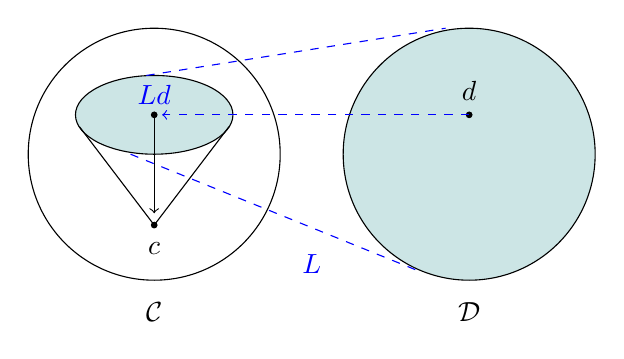
\begin{tikzpicture}
  \def\Xa{2.0};
  \def\Xb{-2.0};
  
  \def\Ytip{-0.9};
  \def\Yo{0.5}; % oval
  \def\Yb{-2.0}; % labels
         \draw (\Xa, 0)[fill=blue!50!green!20]  ellipse (1.6 and 1.6);
         \draw (\Xb , 0) ellipse (1.6 and 1.6);
         % oval
         \draw (\Xb , \Yo)[fill=blue!50!green!20] ellipse (1 and 0.5);
         
        % apex
        \filldraw (\Xb, \Ytip) circle (1pt);
        \node at ( \Xb, \Ytip - 0.3) { $c$ };
        
        % image
        \filldraw (\Xa, \Yo) circle (1pt);
        \node at ( \Xa, \Yo + 0.3) { $d$ };
        
	% middle of the cone
	\draw[->] (\Xb, \Yo) -- (\Xb, \Ytip + 0.15);
        	% sides of the cone
	\draw (\Xb, \Ytip) -- (\Xb + 0.95, \Yo - 0.15);
	\draw (\Xb, \Ytip) -- (\Xb - 0.95, \Yo - 0.15);

        % categories
        \node at (\Xa, \Yb) { $\mathcal D$ };
        \node at (\Xb, \Yb) { $\mathcal C$ };
        \node[blue] at (0, \Yb + 0.6) { $L$ };

        % functor middle
        \filldraw (\Xb, \Yo) circle (1pt);
        \node[blue] at ( \Xb, \Yo + 0.25) { $L d$ };
	\draw[->, blue, dashed] (\Xa, \Yo) -- (\Xb + 0.1, \Yo);
	% functor 
	\draw [blue, dashed] (\Xb - 0.1, \Yo + 0.5    )   --   (\Xa - 0.3, \Yo + 1.1);
	\draw [blue, dashed] (\Xb - 0.3, \Yo - 0.5) -- (\Xa - 0.6, \Ytip - 0.6);
\end{tikzpicture}
\]

重要的观察是,这个逗号范畴描述了 $\cat C$ 中的一个余锥。这个余锥的基由那些在 $L$ 的像中且对 $c$ 有畅通视野的对象组成。余锥基中的箭头是 $L/c$ 中的态射。这些正是使余锥的边交换的箭头。
\[
 \begin{tikzcd}
 L d
 \arrow[rd, "f"']
 \arrow[rr, "L h"]
 && L d'
 \arrow[ld, "f'"]
 \\
 &c
  \end{tikzcd}
 \hspace{30pt}
\begin{tikzcd}
 d
 \arrow[rr, "h"]
 && d'
  \end{tikzcd}
\]

然后可以将这个余锥的基投影回 $\cat D$。有一个投影 $\pi_c$,它将 $L/c$ 中的每对 $(d, f)$ 映射回 $d$,从而忘记箭头 $f$。它还将 $L/c$ 中的每个态射映射到 $\cat D$ 中产生它的箭头。这样 $\pi_c$ 定义了 $\cat D$ 中的一个图。这个图的余极限存在,因为我们假设 $\cat D$ 中存在所有余极限。让我们称这个余极限为 $t_c$:
\[ t_c = \text{colim}\; \pi_c \]

\[
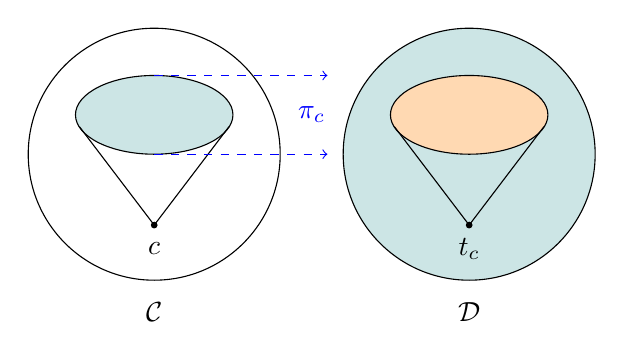
\begin{tikzpicture}
  \def\Xa{2.0};
  \def\Xb{-2.0};
  
  \def\Ytip{-0.9};
  \def\Yo{0.5}; % oval
  \def\Yb{-2.0}; % labels
         \draw (\Xa, 0)[fill=blue!50!green!20]   ellipse (1.6 and 1.6);
         \draw (\Xb , 0) ellipse (1.6 and 1.6);
         % oval
         \draw (\Xb , \Yo)[fill=blue!50!green!20]  ellipse (1 and 0.5);

        % apex
        \filldraw (\Xb, \Ytip) circle (1pt);
        \node at ( \Xb, \Ytip - 0.3) { $c$ };
                
        	% sides of the cone
	\draw (\Xb, \Ytip) -- (\Xb + 0.95, \Yo - 0.15);
	\draw (\Xb, \Ytip) -- (\Xb - 0.95, \Yo - 0.15);

         % second oval
         \draw (\Xa , \Yo) [fill=orange!30]  ellipse (1 and 0.5);
          
        % apex
        \filldraw (\Xa, \Ytip) circle (1pt);
        \node at ( \Xa, \Ytip - 0.3) { $t_c$ };

        	% sides of the cone
	\draw (\Xa, \Ytip) -- (\Xa + 0.95, \Yo - 0.15);
	\draw (\Xa, \Ytip) -- (\Xa - 0.95, \Yo - 0.15);

        % categories
        \node at (\Xa, \Yb) { $\mathcal D$ };
        \node at (\Xb, \Yb) { $\mathcal C$ };
        \node[blue] at (0, \Yo) { $\pi_c$ };

	% functor 
	\draw [->, blue, dashed] (\Xb, \Yo + 0.5) --  (\Xb + 2.2, \Yo + 0.5);
	\draw [->, blue, dashed] (\Xb, \Yo - 0.5)  -- (\Xb + 2.2, \Yo - 0.5);
\end{tikzpicture}
\]

让我们看看是否可以使用这个 $t_c$ 来构造 $L/c$ 中的终端对象。我们必须找到一个箭头,让我们称之为 $\varepsilon_c \colon L t_c \to c$,使得对 $\langle t_c, \varepsilon_c \rangle$ 是 $L/c$ 中的终端对象。

注意,$L$ 将 $\pi_c$ 生成的图映射回由 $L/c$ 定义的余锥的基。投影 $\pi_c$ 所做的不过是忽略这个余锥的边,保持其基不变。

我们现在在 $\cat C$ 中有两个具有相同基的余锥:原始的以 $c$ 为顶点的余锥和通过将 $L$ 应用于 $\cat D$ 中的余锥得到的新余锥。由于 $L$ 保持余极限,新余锥的余极限是 $L t_c$——余极限 $t_c$ 的像:

\[ \text{colim} \; (L \circ \pi_c) = L ( \text{colim} \; \pi_c) = L t_c\]

通过通用构造,我们推断必须存在一个从余极限 $L t_c$ 到 $c$ 的唯一余锥态射。这个态射,我们称之为 $\varepsilon_c$,使所有相关的三角形交换。

剩下要证明的是 $\langle t_c, \varepsilon_c \rangle$ 是 $L/c$ 中的终端对象,即对于任何 $\langle d, f \colon L d \to c \rangle$,存在一个唯一的逗号范畴态射 $h \colon d \to t_c$,使得以下三角形交换:

\[
 \begin{tikzcd}
 L d
 \arrow[rd, "f"']
 \arrow[rr, dashed, "L h"]
 && L t_c
 \arrow[ld, red, "\varepsilon_c"]
 \\
 &c
  \end{tikzcd}
\]

注意,任何这样的 $d$ 自动成为 $\pi_c$ 生成的图的一部分(它是 $\pi_c$ 作用于 $\langle d, f \rangle$ 的结果)。我们知道 $t_c$ 是 $\pi_c$ 图的极限。因此在极限余锥中必须有一条从 $d$ 到 $t_c$ 的线。我们选择这条线作为我们的 $h$。

\[
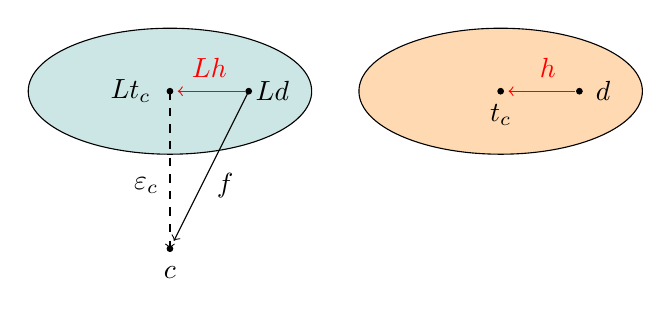
\begin{tikzpicture}
  \def\Xa{2.1};
  \def\Xb{-2.1};
  
  \def\Ytip{0};
  \def\Ybot{-2};
  \def\Yo{0}; % oval
  \def\Yf{-1.2}; % label
         % first oval
         \draw (\Xb , \Yo)[fill=blue!50!green!20]  ellipse (1.8 and 0.8);

         % second oval
         \draw (\Xa , \Yo) [fill=orange!30]  ellipse (1.8 and 0.8);
          
        % apex L tc
        \filldraw (\Xb, \Ytip) circle (1pt);
        \node at ( \Xb - 0.5, \Ytip) { $L t_c$ };
        
        % apex c
        \filldraw (\Xb, \Ybot) circle (1pt);
        \node at ( \Xb, \Ybot - 0.3) { $c$ };
                
        	% sides of the cone L h
	\draw[red, ->]  (\Xb + 0.95, \Yo) -- (\Xb + 0.1, \Ytip);
	\node[red] at (\Xb + 0.5, \Ytip + 0.3) {$L h$};

        % apex tc
        \filldraw (\Xa, \Ytip) circle (1pt);
        \node at ( \Xa, \Ytip - 0.3) { $t_c$ };

        	% sides of the cone h
	\draw [->, red] (\Xa + 0.95, \Yo) -- (\Xa + 0.1, \Ytip);
	\node[red] at ( \Xa + 0.6, \Ytip + 0.3) { $h$ };
	
	% d
        \filldraw (\Xa + 1, \Yo) circle (1pt);
        \node at ( \Xa + 1.3, \Yo) { $d$ };

	% L d
        \filldraw (\Xb + 1, \Yo) circle (1pt);
        \node at ( \Xb + 1.3, \Yo) { $L d$ };
        
        % f
        \draw[->] (\Xb + 1, \Yo) to (\Xb + 0.05, \Ybot + 0.1);
        \node at (\Xb + 0.7, \Yf) {$f$};
        
        % epsilon
        \draw[->, dashed] (\Xb, \Ytip) -- (\Xb, \Ybot);
        \node at (\Xb - 0.3, \Yf) {$\varepsilon_c$};

\end{tikzpicture}
\]
交换条件随后由 $\varepsilon_c$ 作为两个余锥之间的态射得出。它是唯一的余锥态射,因为 $\cat D$ 是一个预序。

这证明了对于每个 $c$ 都存在一个通用箭头 $\langle t_c, \varepsilon_c \rangle$,因此我们有一个函子 $R$,定义为 $R c = t_c$,它是 $L$ 的右伴随。

\end{document}

\subsection{解集条件}

先前证明的问题在于,在大多数实际情况下,逗号范畴(comma category)是大的:它们的对象不构成一个集合。但也许我们可以通过选择一个更小但具有代表性的对象和箭头集来近似逗号范畴?

为了选择对象,我们将使用从某个索引集 $I$ 的映射。我们定义一组对象 $d_i$,其中 $i \in I$。由于我们试图近似逗号范畴 $L/c$,我们选择对象以及箭头 $f_i \colon L d_i \to c$。

逗号范畴的相关部分被编码在满足交换条件的对象之间的态射中。我们可以尝试将这个条件专门化,使其仅适用于我们的对象族,但这还不够。我们必须找到一种方法来探测逗号范畴的所有其他对象。

为此,我们将交换条件重新解释为通过某个对 $\langle d_i, f_i \rangle$ 分解任意 $f \colon L d \to c$ 的配方:
\[
 \begin{tikzcd}
 L d
 \arrow[rd, "f"']
 \arrow[rr, "L h"]
 && \textcolor{red}{L d_i}
 \arrow[ld, red, "f_i"]
 \\
 &c
  \end{tikzcd}
\]

一个\index{解集}\emph{解集}(solution set)是一组由集合 $I$ 索引的对 $\langle d_i, f_i \colon L d_i \to c \rangle$,可以用来分解任何对 $\langle d, f \colon L d \to c \rangle$。这意味着存在一个索引 $i \in I$ 和一个箭头 $h \colon d \to d_i$,使得 $f$ 被分解为:
\[ f = f_i \circ L h \]

表达这个性质的另一种方式是,在逗号范畴 $L/c$ 中存在一个\index{弱终集}\emph{弱终集}(weakly terminal set)。弱终集的性质是,对于范畴中的任何对象,都存在一个态射到该集合中的至少一个对象。

之前我们已经看到,对于每个 $c$,在逗号范畴 $L/c$ 中存在终对象足以定义伴随。事实证明,我们可以使用解集实现相同的目标。

Freyd 伴随函子定理的假设指出,我们有一个保持余极限的函子 $L \colon \cat D \to \cat C$,来自一个小余完备范畴。这两个条件都与\emph{小}图相关。如果我们能为每个 $c$ 选择一个解集 $\langle d_i, f_i \colon L d_i \to c \rangle$,则右伴随 $R$ 存在。不同 $c$ 的解集可能不同。

我们之前已经看到,在余完备范畴中,弱终集的存在足以定义一个终对象。在我们的情况下,这意味着对于任何 $c$,我们可以构造从 $L$ 到 $c$ 的通用箭头。而这足以定义整个伴随。

伴随函子定理的对偶版本可以用来构造左伴随。

\subsection{去函数化(Defunctionalization)}

每种编程语言都允许我们定义函数,但并非所有语言都支持高阶函数(将函数作为参数的函数、返回函数的函数,或由函数构造的数据类型)或匿名函数(又称lambda函数)。事实证明,即使在这样的语言中,也可以通过称为去函数化的过程来实现高阶函数。该技术基于伴随函子定理(adjoint functor theorem)。此外,当传递函数不切实际时(例如在分布式系统中),也可以使用去函数化。

去函数化的核心思想是将函数类型定义为积的右伴随。
\[ \cat C(e \times a, b) \cong \cat C(e, b^a) \]
伴随函子定理可用于近似这个伴随。

一般来说,任何有限程序只能有有限数量的函数定义。这些函数(连同它们捕获的环境)构成了我们可以用来构造函数类型的解集。在实践中,我们只对那些作为其他函数的参数或返回值的函数子集进行此操作。

高阶函数的一个典型应用是在延续传递风格(continuation passing style)中。例如,以下是一个计算列表元素和的函数。但它不是直接返回和,而是调用延续\hask{k}并传递结果:
\begin{haskell}
sumK :: [Int] -> (Int -> r) -> r
sumK [] k = k 0
sumK (i : is) k =
  sumK is (\s -> k (i + s))
\end{haskell}
如果列表为空,函数将调用延续并传递零。否则,它递归调用自身,传递两个参数:列表的尾部\hask{is},以及一个新的延续:
\begin{haskell}
\s -> k (i + s)
\end{haskell}
这个新延续调用之前的延续\hask{k},并传递列表头部与其参数\hask{s}(即累加和)的和。

注意这个lambda是一个闭包:它是一个单变量\hask{s}的函数,但它也可以访问其环境中的\hask{k}和\hask{i}。

为了提取最终的和,我们使用平凡的延续(即恒等函数)调用递归函数:
\begin{haskell}
sumList :: [Int] -> Int
sumList as = sumK as (\i -> i)
\end{haskell}

匿名函数很方便,但没有什么能阻止我们使用命名函数。然而,如果我们想要提取延续,就必须显式传递环境。

例如,我们可以将第一个lambda:
\begin{haskell}
\s -> k (i + s)
\end{haskell}
替换为函数\hask{more},但必须显式传递对\hask{(i, k)}作为类型为\hask{(Int, Int -> r)}的环境:
\begin{haskell}
more :: (Int, Int -> r) -> Int -> r
more (i, k) s = k (i + s)
\end{haskell}
另一个lambda(即恒等函数)使用空环境,因此它变为:
\begin{haskell}
done :: Int -> Int
done i = i
\end{haskell}
以下是使用这两个命名函数的算法实现:
\begin{haskell}
sumK' :: [Int] -> (Int -> r) -> r
sumK' [] k = k 0
sumK' (i : is) k =
  sumK' is (more (i, k))
\end{haskell}

\begin{haskell}
sumList :: [Int] -> Int
sumList is = sumK' is done
\end{haskell}

事实上,如果我们只关心计算和,可以将多态类型\hask{r}替换为\hask{Int},而无需其他更改。

此实现仍然使用高阶函数。为了消除它们,我们必须分析将函数作为参数传递的含义。这样的函数只能以一种方式使用:它可以应用于其参数。函数类型的这一性质表示为柯里化伴随的余单位(counit):
\[ \varepsilon \colon b^a \times a \to b \]
或在Haskell中,作为一个高阶函数:
\begin{haskell}
apply :: (a -> b, a) -> b
\end{haskell}
这次我们感兴趣的是从基本原理构造余单位。我们已经看到,这可以通过逗号类别(comma category)实现。在我们的例子中,积函子$L_a = (-) \times a$的逗号类别的一个对象是一对
\[(e, f \colon (e \times a) \to b) \]
或在Haskell中:
\begin{haskell}
data Comma a b e = Comma e ((e, a) -> b)
\end{haskell}
此类别中$(e, f)$和$(e', f')$之间的态射是一个箭头$h \colon e \to e'$,它满足交换条件:
\[ f' \circ h = f \]
我们将此态射解释为将环境$e$“缩减”到$e'$。箭头$f'$能够使用由$h (e)$给出的潜在更小的环境生成相同类型$b$的输出。例如,$e$可能包含与从$a$计算$b$无关的变量,而$h$将它们投影出去。

\[
 \begin{tikzcd}
 e \times a
 \arrow[rd, "f"']
 \arrow[rr, "h \times a"]
 && e' \times a
 \arrow[ld, "f'"]
 \\
 &b
  \end{tikzcd}
 \hspace{30pt}
\begin{tikzcd}
 e
 \arrow[rr, "h"]
 && e'
  \end{tikzcd}
\]

事实上,我们在定义\hask{more}和\hask{done}时执行了这种缩减。原则上,我们可以将尾部\hask{is}传递给这两个函数,因为它在调用点是可访问的。但我们知道它们不需要它。

使用Freyd定理,我们可以将函数对象$a \to b$定义为由逗号类别定义的图的余极限(colimit)。这样的余极限本质上是所有环境的巨大余积(coproduct),模由逗号类别态射给出的标识。这种标识将$a \to b$所需的环境缩减到最低限度。

在我们的例子中,我们感兴趣的延续是函数\hask{Int -> Int}。事实上,我们并不感兴趣生成通用的函数类型\hask{Int -> Int};只是生成能够容纳我们两个函数\hask{more}和\hask{done}的最小函数类型。我们可以通过创建一个非常小的解集来实现。

在我们的例子中,解集由$(e_i, f_i \colon e_i \times a \to b)$对组成,使得任何对$(e, f \colon e \times a \to b)$都可以通过其中一个$f_i$进行因式分解。更准确地说,我们感兴趣的唯二环境是\hask{(Int, Int ->Int)}(用于\hask{more})和空环境\hask{()}(用于\hask{done})。

原则上,我们的解集应允许对逗号类别的每个对象进行因式分解,即类型为:
\begin{haskell}
(e, (e, Int) -> Int)
\end{haskell}
的对,但这里我们只对两个特定函数感兴趣。此外,我们不关心表示的唯一性,因此,我们不会使用余极限(如我们在伴随函子定理中所做的那样),而是仅使用所有感兴趣环境的余积。我们最终得到以下数据类型,它是我们感兴趣的两个环境\hask{()}和\hask{(Int, Int -> Int)}的和。我们最终得到类型:
\begin{haskell}
data Kont = Done | More Int Kont
\end{haskell}
注意,我们已将环境的\hask{Int->Int}部分递归编码为\hask{Kont}。因此,我们也消除了将函数作为数据构造器参数的需要。

如果你仔细查看这个定义,你会发现它是一个\hask{Int}列表的定义,模一些重命名。每次调用\hask{More}都会将另一个整数推入\hask{Kont}栈。这种解释与我们的直觉一致,即递归算法需要某种运行时栈。

我们现在准备实现我们对伴随余单位的近似。它由两个函数的主体组成,并理解递归调用也通过\hask{apply}进行:
\begin{haskell}
apply :: (Kont, Int) -> Int
apply (Done, i) = i
apply (More i k, s) = apply (k, i + s)
\end{haskell}
将其与我们之前的代码进行比较:
\begin{haskell}
done i = i
more (i, k) s = k (i + s)
\end{haskell}

现在,主算法可以重写为不包含任何高阶函数或lambda的形式:
\begin{haskell}
sumK'' :: [Int] -> Kont -> Int
sumK'' [] k = apply (k, 0)
sumK'' (i : is) k = sumK'' is (More i k)
\end{haskell}

\begin{haskell}
sumList'' is = sumK'' is Done
\end{haskell}

去函数化的主要优点是它可以在分布式环境中使用。只要远程函数的参数是数据结构而不是函数,就可以将其序列化并通过网络发送。接收方只需访问\hask{apply}即可。

\section{自由/遗忘伴随}
伴随中的两个函子扮演着不同的角色:伴随的图示并不对称。这一点在自由/遗忘伴随的情况下体现得尤为明显。

遗忘函子(forgetful functor)是一种“遗忘”其源范畴某些结构的函子。这并不是一个严格的定义,但在大多数情况下,被遗忘的结构是显而易见的。通常,目标范畴就是集合范畴,它被认为是无结构的典范。在这种情况下,遗忘函子的结果被称为“底层”集合,而函子本身通常记为$U$。

更准确地说,我们说一个函子遗忘\emph{结构},如果hom集的映射不是满射的,也就是说,目标hom集中存在没有对应源hom集中箭头的箭头。直观上,这意味着源中的箭头需要保留某些结构,因此它们的数量较少;而这些结构在目标中是不存在的。

遗忘函子的左伴随被称为\emph{自由函子}。

\[
 \begin{tikzcd}
F x
\arrow[d, bend right, red, dashed]
\arrow[d, dashed]
\arrow[d, bend left, blue, dashed]
  &&
  x
\arrow[d, bend right, red, dashed]
\arrow[d, dashed]
\arrow[d, bend left, blue, dashed]
 \arrow[ll, bend right, "F"']
 \\
y
   \arrow[rr, bend right, "U"']
 &&
 U y
  \end{tikzcd}
\]

自由/遗忘伴随的一个经典例子是自由幺半群的构造。

\subsection{幺半群范畴}
幺半群范畴$\mathcal{C}$中的幺半群形成它们自己的范畴$\mathbf{Mon}(\mathcal{C})$。其对象是幺半群,其箭头是$\mathcal{C}$中保留幺半群结构的箭头。

以下图示解释了$f$作为幺半群态射的含义,从幺半群$(M_1, \eta_1, \mu_1)$到幺半群$(M_2, \eta_2, \mu_2)$:
\[
 \begin{tikzcd}
 & M_1
 \arrow[dd, "f"]
 & M_1 \otimes M_1
 \arrow[l, "\mu_1"]
 \arrow[dd, "f \otimes f"]
 \\
 I
 \arrow[ru, "\eta_1"]
 \arrow[rd, "\eta_2"']
 \\
 & M_2
 & M_2 \otimes M_2
 \arrow[l, "\mu_2"]
  \end{tikzcd}
\]
幺半群态射$f$必须将单位元映射到单位元,这意味着:
\[ f \circ \eta_1 = \eta_2 \]
并且它必须将乘法映射到乘法:
\[ f \circ \mu_1 = \mu_2 \circ (f \otimes f)\]
记住,张量积$\otimes$是函子性的,因此它可以提升箭头对,如$f \otimes f$。

特别地,范畴$\mathbf{Set}$是幺半群的,其笛卡尔积和终端对象提供了幺半群结构。

特别地,$\mathbf{Set}$中的幺半群是具有额外结构的集合。它们形成自己的范畴$\mathbf{Mon}(\mathbf{Set})$,并且存在一个遗忘函子$U$,它简单地将幺半群映射到其元素的集合。当我们说幺半群是一个集合时,我们指的是底层集合。

\subsection{自由幺半群}

我们希望构造自由函子
\[ F \colon \mathbf{Set} \to \mathbf{Mon}(\mathbf{Set})\]
它是遗忘函子$U$的伴随。

我们从任意集合$X$和任意幺半群$m$开始。在伴随的右侧,我们有从$X$到$U m$的函数集合。在左侧,我们有一组高度受限的结构保持的幺半群态射,从$F X$到$m$。这两个hom集如何同构?

在$\mathbf{Mon}(\mathbf{Set})$中,幺半群是元素的集合,幺半群态射是这些集合之间的函数,满足额外的约束:保留单位元和乘法。

另一方面,$\mathbf{Set}$中的箭头只是没有额外约束的函数。因此,一般来说,幺半群之间的箭头比它们的底层集合之间的箭头要少。

\[
 \begin{tikzcd}
F X
\arrow[d, bend right, red, dashed]
\arrow[d, dashed]
\arrow[d, bend left, blue, dashed]
  &&
X
\arrow[d, bend right, red, dashed]
\arrow[d, dashed]
\arrow[d, bend left, blue, dashed]
 \arrow[ll, bend right, "F"']
 \\
m
   \arrow[rr, bend right, "U"']
 &&
 U m
  \end{tikzcd}
\]

这里的想法是:如果我们想要在箭头之间有一一对应,我们希望$F X$比$X$大得多。这样,从它到$m$的函数会更多——即使排除了那些不保留结构的函数,我们仍然有足够的函数来匹配每个函数$f \colon X \to U m$。

我们将从集合$X$开始构造幺半群$F X$,并逐步添加更多元素。我们将初始集合$X$称为$F X$的\index{幺半群的生成元}\emph{生成元}。我们将从原始函数$f$开始构造一个幺半群态射$g \colon F X \to m$,并将其扩展到更多的元素上。

在生成元上,$x \in X$,$g$与$f$相同:
\[ g x = f x \]

由于$F X$应该是一个幺半群,它必须有一个单位元。我们不能选择一个生成元作为单位元,因为它会对$g$的已经由$f$固定的部分施加约束——它必须将其映射到$m$的单位元$e'$。因此,我们只需在$F X$中添加一个额外的元素$e$,并将其称为单位元。我们将通过说它被映射到$m$的单位元$e'$来定义$g$在它上的作用:
\[ g e = e' \]

我们还必须在$F X$中定义幺半群乘法。让我们从两个生成元$a$和$b$的乘积开始。乘法的结果不能是另一个生成元,因为这将再次约束$g$的已经由$f$固定的部分——乘积必须被映射到乘积。因此,我们必须使所有生成元的乘积成为$F X$的新元素。同样,$g$在这些乘积上的作用是固定的:
\[ g (a \cdot b)  = g a \cdot g b\]

继续这个构造,任何新的乘法都会产生$F X$的新元素,除非它可以通过应用幺半群定律简化为现有元素。例如,新的单位元$e$乘以生成元$a$必须等于$a$。但我们已经确保$e$被映射到$m$的单位元,因此乘积$g e \cdot g a$自动等于$g a$。

另一种看待这个构造的方式是将集合$X$视为一个字母表。$F X$的元素就是来自这个字母表的字符串。生成元是单字母字符串,如“$a$”、“$b$”等。单位元是空字符串“”。乘法是字符串连接,因此“$a$”乘以“$b$”是一个新字符串“$ab$”。连接自动是结合的和单位的,空字符串作为单位元。

自由函子的直觉是它们“自由地”生成结构,即“没有额外的约束”。它们也以惰性的方式生成:它们不执行操作,而是记录操作。它们创建了可以在以后由特定解释器执行的通用领域特定程序。

自由幺半群“记住稍后执行乘法”。它将乘法的参数存储在字符串中,但不执行乘法。它只能根据通用幺半群定律简化其记录。例如,它不必存储乘以单位元的命令。由于结合性,它也可以“跳过括号”。

\begin{exercise}
自由幺半群伴随$F \dashv U$的单位元和余单位元是什么?
\end{exercise}

\subsection{编程中的自由幺半群}

在Haskell中,幺半群使用以下类型类定义:
\begin{haskell}
class Monoid m where
  mappend :: m -> m -> m
  mempty  :: m
\end{haskell}
这里,\hask{mappend}是乘积映射的柯里化形式:\hask{(m, m) -> m}。\hask{mempty}元素对应于从终端对象(幺半群范畴的单位元)的箭头,或者简单地说是\hask{m}的一个元素。

由某个类型\hask{a}生成的自由幺半群,作为生成元的集合,由列表类型\hask{[a]}表示。空列表作为单位元;幺半群乘法实现为列表连接,传统上以中缀形式书写:
\begin{haskell}
(++) :: [a] -> [a] -> [a]
(++) []     ys = ys
(++) (x:xs) ys = x : xs ++ ys
\end{haskell}
列表是\hask{Monoid}的一个实例:
\begin{haskell}
instance Monoid [a] where
  mempty = []
  mappend = (++)
\end{haskell}

为了证明它是一个自由幺半群,我们必须能够从\hask{a}的列表构造一个幺半群态射到任意幺半群\hask{m},前提是我们有一个(无约束的)从\hask{a}到(底层集合)\hask{m}的映射。我们无法在Haskell中表达所有这些,但我们可以定义函数:
\begin{haskell}
foldMap :: Monoid m => (a -> m) -> ([a] -> m)
foldMap f = foldr mappend mempty . fmap f
\end{haskell}
这个函数使用\hask{f}将列表的元素转换为幺半群值,然后使用\hask{mappend}从单位元\hask{mempty}开始折叠它们。

很容易看出,空列表被映射到幺半群单位元。不难看出,两个列表的连接被映射到结果的幺半群乘积。因此,\hask{foldMap}确实是一个幺半群态射。

根据自由幺半群作为乘法操作的领域特定程序的直觉,\hask{foldMap}提供了这个程序的\emph{解释器}。它执行所有被推迟的乘法。请注意,同一个程序可以根据具体幺半群和函数\hask{f}的选择以多种不同的方式解释。

我们将在关于代数的章节中再次讨论作为列表的自由幺半群。

\begin{exercise}
编写一个程序,接受一个整数列表,并以两种不同的方式解释它:一次使用整数的加法幺半群,一次使用整数的乘法幺半群。
\end{exercise}

\section{伴随关系的范畴}
我们可以通过利用定义伴随关系的函子的复合来定义伴随关系的复合。两个伴随关系 $L \dashv R$ 和 $L' \dashv R'$ 是可复合的,如果它们共享中间的范畴:
\[
 \begin{tikzcd}
  \mathcal{C}
  \arrow[rr, bend right, "R'"']
  &&
  \mathcal{D}
  \arrow[ll, bend right, "L'"']
    \arrow[rr, bend right, "R"']
&&
  \mathcal{E}
  \arrow[ll, bend right, "L"']
 \end{tikzcd}
\]
通过复合函子,我们得到一个新的伴随关系 $(L' \circ L) \dashv (R \circ R')$。

实际上,让我们考虑 hom-集:
\[ \mathcal{C}(L' (L e), c) \]
利用 $L' \dashv R'$ 伴随关系,我们可以将 $L'$ 转置到右边,它变为 $R'$:
\[ \mathcal{D}(L e, R' c) \]
然后利用 $L \dashv R$,我们可以类似地转置 $L$:
\[ \mathcal{E}( e, R(R' c)) \]
结合这两个同构,我们得到复合的伴随关系:
\[ \mathcal{C}((L' \circ L) e, c) \cong \mathcal{E}( e, (R \circ R') c)\]

由于函子的复合是结合的,伴随关系的复合也是结合的。容易看出,一对恒等函子形成一个平凡的伴随关系,它在伴随关系的复合中充当恒等元。因此,我们可以定义一个范畴 $\mathbf{Adj}(\mathbf{Cat})$,其中对象是范畴,箭头是伴随关系(按照惯例,指向左伴随的方向)。

伴随关系可以纯粹用函子和自然变换来定义,即 2-范畴 $\mathbf{Cat}$ 中的 1-细胞和 2-细胞。$\mathbf{Cat}$ 并没有什么特别之处,事实上,伴随关系可以在任何 2-范畴中定义。此外,伴随关系的范畴本身也是一个 2-范畴。

\section{抽象层次}

范畴论(Category theory)是关于知识结构化的理论。特别是,它可以应用于范畴论自身的知识。因此,我们在范畴论中看到了大量抽象层次的混合。我们在一个层次上看到的结构可以被分组为更高层次的结构,这些结构展现出更高层次的结构,依此类推。

在编程中,我们习惯于构建抽象层次结构。值被分组为类型,类型被分组为种类(kinds)。操作值的函数与操作类型的函数被区别对待。我们经常使用不同的语法来区分抽象层次。但在范畴论中并非如此。

从范畴论的角度来看,一个集合可以被描述为一个离散范畴(discrete category)。集合的元素是这个范畴的对象,除了必须的恒等态射(identity morphisms)外,它们之间没有箭头。

然后,同一个集合可以被视为范畴 $\mathbf{Set}$ 中的一个对象。这个范畴中的箭头是集合之间的函数。

范畴 $\mathbf{Set}$ 本身又是范畴 $\mathbf{Cat}$ 中的一个对象。$\mathbf{Cat}$ 中的箭头是函子(functors)。

任意两个范畴 $\mathcal{C}$ 和 $\mathcal{D}$ 之间的函子是函子范畴 $[\mathcal{C}, \mathcal{D}]$ 中的对象。这个范畴中的箭头是自然变换(natural transformations)。

我们可以在函子范畴、积范畴(product categories)、对偶范畴(opposite categories)等之间定义函子,如此无限延伸。

完成这个循环,每个范畴中的 hom-集(hom-sets)都是集合。我们可以在它们之间定义映射和同构(isomorphisms),跨越不同的范畴。伴随(adjunctions)之所以可能,是因为我们可以比较存在于不同范畴中的 hom-集。

\end{document}
